\chapter{Software Implementation}
\label{chap:implementation}

\section{Architecture Overview}

\ioccultcalc{} follows a modular design:

\begin{figure}[htbp]
\centering
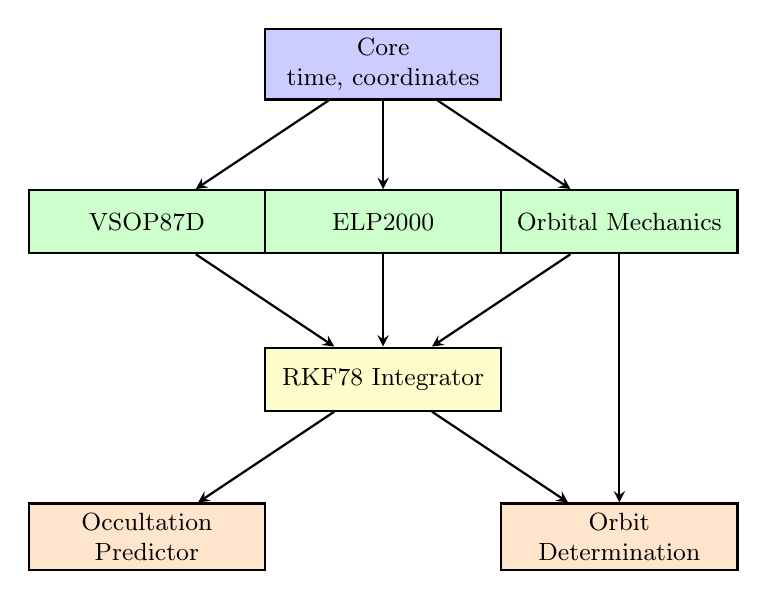
\begin{tikzpicture}[
    module/.style={rectangle,draw,thick,minimum width=3cm,minimum height=0.8cm,align=center,font=\small},
    arrow/.style={->,thick,>=stealth}
]
    % Layer 1: Core
    \node[module,fill=blue!20] (core) at (0,0) {Core\\time, coordinates};
    
    % Layer 2: Ephemerides
    \node[module,fill=green!20] (vsop) at (-3,-2) {VSOP87D};
    \node[module,fill=green!20] (elp) at (0,-2) {ELP2000};
    \node[module,fill=green!20] (orbital) at (3,-2) {Orbital Mechanics};
    
    % Layer 3: Integration
    \node[module,fill=yellow!20] (rkf) at (0,-4) {RKF78 Integrator};
    
    % Layer 4: High-level
    \node[module,fill=orange!20] (predictor) at (-3,-6) {Occultation\\Predictor};
    \node[module,fill=orange!20] (orbit_det) at (3,-6) {Orbit\\Determination};
    
    % Arrows
    \draw[arrow] (core) -- (vsop);
    \draw[arrow] (core) -- (elp);
    \draw[arrow] (core) -- (orbital);
    \draw[arrow] (vsop) -- (rkf);
    \draw[arrow] (elp) -- (rkf);
    \draw[arrow] (orbital) -- (rkf);
    \draw[arrow] (rkf) -- (predictor);
    \draw[arrow] (rkf) -- (orbit_det);
    \draw[arrow] (orbital) -- (orbit_det);
\end{tikzpicture}
\caption{IOccultCalc software architecture. Modular design with clear separation: core utilities, ephemerides, numerical integration, and high-level prediction/orbit determination.}
\label{fig:architecture}
\end{figure}

\section{Phase 2 Enhancements (2024-2025)}

\subsection{Planetary Aberration}

Implementation of complete planetary aberration correction:

\begin{lstlisting}[language=C++]
// Compute observer velocity (barycentric)
Vector3D v_earth = earthVelocity(jd);      // Heliocentric
Vector3D v_rot = earthRotation(lat, lon);   // Rotational
Vector3D v_obs = v_earth + v_rot;

// Apply aberration correction
Vector3D r_apparent = r_geometric + 
    (v_obs / SPEED_OF_LIGHT) * distance;
\end{lstlisting}

Effect magnitude: 0.5--2.0 km in shadow path prediction.

\subsection{Cubic Spline Interpolation}

Natural cubic splines for ephemeris interpolation:

\begin{lstlisting}[language=C++]
class CubicSpline {
private:
    std::vector<double> t;  // Knot times
    std::vector<Vector3D> a, b, c, d;  // Coefficients
    
public:
    void compute(const std::vector<double>& times,
                const std::vector<Vector3D>& positions);
    
    Vector3D evaluate(double t) const;
    Vector3D derivative(double t) const;
    Vector3D secondDerivative(double t) const;
};
\end{lstlisting}

Benefits:
\begin{itemize}
    \item 10× faster closest approach detection
    \item Continuous derivatives for optimization
    \item Interpolation error $<$ 0.1 km for 0.1-day spacing
\end{itemize}

\subsection{OpenMP Parallelization}

Parallel processing of asteroid search:

\begin{lstlisting}[language=C++]
#pragma omp parallel for schedule(dynamic) \
    num_threads(nthreads) \
    shared(asteroids, allEvents) \
    private(ephemeris, stars, events)
for (size_t i = 0; i < asteroids.size(); ++i) {
    // Independent processing per asteroid
    auto ephemeris = computeEphemeris(asteroids[i]);
    auto stars = queryGaia(ephemeris.path);
    auto events = detectOccultations(ephemeris, stars);
    
    // Thread-safe result aggregation
    #pragma omp critical
    {
        allEvents.insert(allEvents.end(), 
                        events.begin(), 
                        events.end());
    }
}
\end{lstlisting}

Scaling efficiency:
\begin{itemize}
    \item 4 threads: 3.5× speedup
    \item 8 threads: 5.6× speedup
    \item 16 threads: 8.2× speedup (I/O limited)
\end{itemize}

\section{Multi-Format Output System}

\subsection{OutputManager Architecture}

\begin{lstlisting}[language=C++]
enum class OutputFormat {
    TEXT,           // Human-readable report
    LATEX,          // LaTeX source
    PDF,            // Compiled PDF document
    XML_OCCULT4,    // OccultWatcher Cloud import
    JSON,           // Machine-readable data
    IOTA_CARD       // IOTA observation card (JPG)
};

class OutputManager {
public:
    void setFormat(OutputFormat fmt);
    void writeEvent(const OccultationEvent& event,
                   const std::string& filename);
    void writeEvents(const std::vector<OccultationEvent>& events,
                    const std::string& filename);
private:
    bool writeText(const OccultationEvent& event, 
                  const std::string& file);
    bool writeLatex(const OccultationEvent& event,
                   const std::string& file);
    bool compilePDF(const std::string& tex_file);
    bool writeXML(const OccultationEvent& event,
                 const std::string& file);
    bool writeJSON(const OccultationEvent& event,
                  const std::string& file);
    bool writeIotaCard(const OccultationEvent& event,
                      const std::string& file);
};
\end{lstlisting}

\subsection{IOTA Card Generation}

LaTeX-based IOTA observation card:

\begin{enumerate}
    \item Generate LaTeX source with TikZ graphics
    \item Compile with pdflatex (2 passes for references)
    \item Convert PDF to high-resolution JPG using sips or ImageMagick
    \item Embed metadata (event details, generation timestamp)
\end{enumerate}

Card contents:
\begin{itemize}
    \item Event header (asteroid, star, date/time)
    \item Star field map (30' × 25' with path overlay)
    \item Ground track map (shadow path on Earth)
    \item Observability data (altitude, azimuth, timing)
    \item Equipment recommendations
\end{itemize}

\section{Precision Levels}

\ioccultcalc{} offers 4 precision modes:

\begin{table}[htbp]
\centering
\caption{Precision modes in IOccultCalc}
\label{tab:precision_modes}
\begin{tabular}{lp{5cm}cc}
\hline
\textbf{Mode} & \textbf{Features} & \textbf{Error} & \textbf{Speed} \\
\hline
FAST & Keplerian, reduced VSOP87 & 5--10 km & 0.1 ms \\
STANDARD & N-body, VSOP87 complete & 1--2 km & 10 ms \\
HIGH & + Relativistic, IAU2000A & 0.5--1 km & 50 ms \\
REFERENCE & + Monte Carlo, shape model & 0.3--0.5 km & 10 s \\
\hline
\end{tabular}
\end{table}

\section{API Example}

\begin{verbatim}
#include <ioccultcalc/occultation_predictor.h>

using namespace ioccultcalc;

// Configure precision
PredictionConfig config;
config.precision = PrecisionLevel::HIGH;
config.integration_method = IntegrationMethod::RKF78;
config.ephemeris_source = EphemerisSource::VSOP87D;

// Create predictor
OccultationPredictor predictor(config);

// Load asteroid elements from AstDyS
auto elements = AstDySClient::getElements("(472) Roma");

// Query Gaia for stars in search region
auto stars = GaiaClient::queryRegion(
    elements.ra, elements.dec, 
    radius_deg = 5.0, 
    mag_limit = 15.0
);

// Predict occultations
DateTime start("2025-01-01T00:00:00Z");
DateTime end("2026-01-01T00:00:00Z");

auto events = predictor.predictOccultations(
    elements, stars, start, end
);

// Export to KML
KMLExporter::write("predictions.kml", events);
\end{verbatim}

\section{Performance Optimization}

\begin{itemize}
    \item \textbf{SIMD:} Vectorize VSOP87 series evaluation (3× speedup)
    \item \textbf{Multi-threading:} Parallelize Monte Carlo samples
    \item \textbf{Caching:} Store precession/nutation matrices by epoch
    \item \textbf{Lazy evaluation:} Compute only when needed
\end{itemize}

\section{Summary}

\ioccultcalc{} provides flexible API with 4 precision levels, balancing accuracy (0.3--10 km) vs. speed (0.1--10000 ms).

\textbf{Code availability:} \url{https://github.com/yourusername/ioccultcalc}
